\documentclass[12pt]{article}

\usepackage[margin=1.3in]{geometry}
\usepackage{amsmath, amsfonts}
\usepackage[english]{babel}
\usepackage{hyperref}
\usepackage{cleveref}
\usepackage{listings}
\usepackage{graphicx}
\usepackage[T1]{fontenc}
\usepackage[utf8]{inputenc}
\usepackage{titling}
\setlength{\droptitle}{-0.6in}

\title{Oblique Decision Tree Induction}
\author{Koen Dercksen - 4215966}
\date{July 27, 2014}

\renewcommand{\arraystretch}{1.5}
\hypersetup{colorlinks=true}
\lstset{basicstyle=\ttfamily}

\begin{document}

\maketitle

\begin{abstract}
Decision tree learning is a commonly used method of creating a classification model in data mining. This report describes an algorithm for building oblique decision trees; decision trees that split data according to a weighted combination of example attributes. Oblique decision trees are meant to be used in numeric problem domains. The algorithm, a derivation of OC1, is described and examined using the Iris flower dataset \cite{Bache+Lichman:2013}.
\end{abstract}

\bigskip

\section{Introduction}
Most decision tree (DT) algorithms create DTs in which each node checks the value of a single attribute; this is especially useful when looking at datasets with discrete values. Univariate tests in numeric datasets split at a certain threshold. The tests in each node are of the form
\begin{align*}
x_i > c
\end{align*}
where $x_i$ is the value of a single attribute and $c$ is a constant. DTs that use this splitting method are referred to as \emph{axis-parallel}, because the tests basically represent axis-parallel hyperplanes in the problem space. Depending on the dataset, axis-parallel splits may or may not be sufficient. These types of splits can be visualized as seen in \cref{fig:axisparallel}.

\begin{figure}[!ht]
\centering
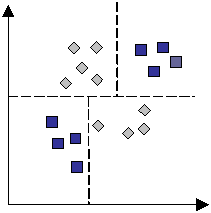
\includegraphics[scale=0.5]{images/axisparallel.png}
\caption{Axis-parallel decision boundaries.}
\label{fig:axisparallel}
\end{figure}

The algorithm examined in this article tests linear combinations of attributes at each node in the DT, creating non-axis-parallel (oblique) hyperplanes in the problem space. Depending on the dataset, this can result in a higher purity split. Assuming that every example has the form $X = x_1, \ldots, x_d, C_j$ where $x_i$ is a real-valued attribute and $C_j$ the class label, oblique DTs consider a test of the form
\begin{align} \label{eq:obliquetest}
\sum\limits_{i = 0}^{d} (a_i x_i) + a_{d + 1} > 0
\end{align}
at every node, where $a_1, \ldots, a_{d + 1}$ are real-valued coefficients. An oblique split visualization can be seen in \cref{fig:obliquesplit}. Recreating axis-parallel splits while using tests of the form specified in \cref{eq:obliquetest} is very easy, since by choosing $a_i = 0$ for every $i$ except one the test becomes univariate (see \cref{app:code} for the implementation).

\begin{figure}[!ht]
\centering
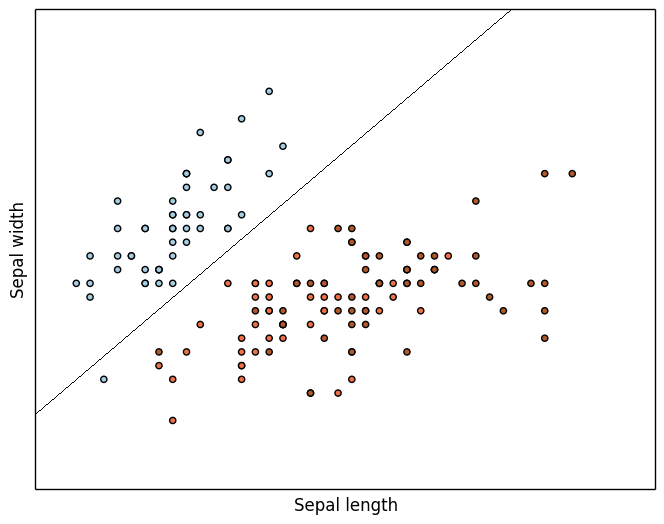
\includegraphics[scale=0.4]{images/sepal_length-sepal_width-withline.png}
\caption{Oblique decision boundary demonstrated on a two-attribute plot of the Iris flower dataset.}
\label{fig:obliquesplit}
\end{figure}

I've implemented an oblique DT classifier, using previous work by Murthy, Kasif and Salzberg \cite{KSM:1994} as a reference.

\section{Decision Tree Induction}
The basic algorithm for top-down DT induction is as follows:
\begin{enumerate}
\item Start with dataset $T$. If all examples in $T$ belong to the same class, stop.
\item Find all tests that divide $T$ into 2 (or more) subsets, and calculate the impurity of each test.
\item Choose the highest purity test.
\item Split $T$ into subsets according to the test found in $3.$ and run the algorithm recursively on each subset.
\end{enumerate}

\subsection{Finding Good Splits}
My version of the oblique DT algorithm initializes every node as the best axis-parallel split before trying to rotate it into a better oblique split. Finding the best axis-parallel split is relatively easy:
\begin{enumerate}
\item Take a dataset $T$ and choose an attribute $i$ to split on (all attributes are considered).
\item Sort $T$ according to each examples value for $x_i$ where $i$ is the attribute you chose.
\item Calculate all midpoints between the sorted $x_i$'s and use those as possible splits.
\item For every possible split $s'$, divide $T$ into subsets according to \cref{eq:obliquetest} where we set all $a = 0$ except for $a_i$, which we set to $s'$, and $a_{d+1}$ which we set to $-s'$. Store the impurity of each such split.
\item Choose the value for $a_i$ that results in the highest purity split.
\end{enumerate}

See \cref{app:code} for the implementation.

Now we have the option to rotate this initial split and keep the new version if it results in a higher purity. Murthy, Kasif and Salzberg refer to this rotation step as \emph{perturbation} \cite{KSM:1994}. Perturbation takes the initial axis-parallel split and tries to optimize every coefficient $a_m$ locally by calculating the best univariate split for attribute $m$ assuming that all $a_i$ where $i \neq m$ are constants. If after perturbing the initial split a higher purity split is achieved, the initial split is replaced with the perturbed split. If the purity of the initial and the perturbed split is the same, the perturbed split replaces the initial split with a certain probability.

My implementation runs the perturbation step 10 times on random attributes. Murthy, Kasif and Salzberg explored more methods of perturbation (50 times random, sequential, best \cite{KSM:1994}) but mentioned that none was uniformly better than the others.

\subsection{Complexity}
When finding oblique splits, considering all possible tests at every node in order to find the best one is not feasible due to complexity reasons. More precisely: assuming a dataset with $n$ examples each containing $d$ attributes, there are $n \cdot d$ unique axis-parallel splits while there are $2^d \cdot {n \choose d}$ unique $d$-dimensional oblique splits (every subset of size $d$ from the $n$ points can create a $d$-dimensional split and each such split can be rotated in $2^d$ directions) \cite{KSM:1994}. Therefore, searching for the best oblique split is much harder than finding the best axis-parallel split.

While testing my implementation, I found that it scaled very badly to larger datasets. The classifier easily fits Iris flower dataset in a normal timeframe, however datasets of sizes akin to $8000x10$ took forever to fit. This might be due to a combination of the problem being hard and a possibly bad implementation.

\subsection{Similar algorithms}
My work is largely based on the paper on OC1 by Murthy, Kasif and Salzberg \cite{KSM:1994}. Their algorithm has a few more fancy things about it that didn't make it into my implementation. For example, OC1 includes two types of randomization to escape local minima that I have left out. I have not implemented pruning either. I left these features out largely due to time constraints.

\section{Results}
I have applied my classifier to the Iris flower dataset. I used 5 runs of 5-fold cross-validation to measure the performance of my implementation. Training and validating every fold took under 10 seconds on average on my computer; your mileage may vary. The results can be seen in \cref{tab:cvresults}. As the table shows, the classifier performs with an average of 92.3\% accuracy when validated using 5-fold cross-validation. I'm fairly certain this percentage would be higher if I had implemented some kind of randomization to avoid local minima.

When training the classifier on the whole dataset and then validating it by predicting the whole dataset again, it reliably achieves 100\% accuracy. This is both good and worrying; the lack of a pruning measure probably results in overfitting, which might make it perform worse in situations where there is unseen data to classify (such as in my main validation method).

I'm quite satisfied with the result of this project. If only I had more time, I'm sure I could have done better, but 92.3\% correctness is not bad.

\section{Possible improvements}
Adding randomization and pruning like in OC1 will likely improve the results of the classifier. Furthermore, porting to another language and/or optimizing the current code might lead to faster fitting of the classifier.

\begin{table}[!ht]
\centering
\begin{tabular}{c|cccccc}
Run nr. & \multicolumn{5}{c}{Error rate} & Avg. error rate \\ \hline
1 & 0.033 & 0.100 & 0.067 & 0.067 & 0.000 & 0.053 \\
2 & 0.033 & 0.067 & 0.133 & 0.067 & 0.100 & 0.080 \\
3 & 0.100 & 0.133 & 0.033 & 0.033 & 0.100 & 0.080 \\
4 & 0.100 & 0.067 & 0.067 & 0.067 & 0.167 & 0.093 \\
5 & 0.167 & 0.167 & 0.067 & 0.067 & 0.033 & 0.080 \\ \hline
~ & ~     & ~     & ~     & ~     & ~     & 0.077
\end{tabular}
\caption{Cross-validation results.}
\label{tab:cvresults}
\end{table}

\appendix
\section{Code listing} \label{app:code}
The full implementation can be found at \href{http://github.com/KDercksen/pyblique}{my Github}. I used \href{http://www.python.org}{Python 3} and various libraries from the \href{http://www.scipy.org}{Scipy stack}. Some interesting functions are listed below.

\subsection{Decision Tree Creation}
\begin{lstlisting}[language=Python]
def __create_decision_tree(self, data):
    if len(data) == 0:
        return -1
    isleaf, leaf = self.__is_leaf_node(data)
    if isleaf:
        return leaf
    else:
        splits = self.__get_all_splits(data)
        index, split = min(enumerate(splits), 
                           key=lambda x: x[1][1])
        # in order to make this oblique, we first 
        # have to build a vector to enable the
        # linear combination split
        sv = np.zeros((len(data[0]),))
        sv[-1] = -split[0]
        sv[index] = 1
        low, high = self.__split_data(data, sv)
        imp = self.metric(low, -1) + self.metric(high, -1)
        # perturb random attributes
        for c in range(10):
            r = randint(0, len(sv) - 1)
            imp, sv = self.__perturb(data, sv, r, imp)
        tree = {"split": sv}
        low, high = self.__split_data(data, sv)
        subtree_low = self.__create_decision_tree(low)
        tree["low"] = subtree_low
        subtree_high = self.__create_decision_tree(high)
        tree["high"] = subtree_high
    return tree
\end{lstlisting}

\subsection{Best Axis-Parallel Split}
This function is called for every attribute.
\begin{lstlisting}[language=Python]
def __best_split_on_attr(self, data, attr):
    # Will return a tuple of (split test, split value).
    split_values = self.__get_splits(data, attr)
    split_evals = {}
    for s in split_values:
        cond = data[:, attr] <= s
        left, right = data[cond], data[~cond]
        split_evals[s] = self.metric(left, -1) + 
                         self.metric(right, -1)
    # Minimize because we're using gini index
    return min(split_evals.items(), key=lambda x: x[1])
\end{lstlisting}

\subsection{Perturbation}
\begin{lstlisting}[language=Python]
def __perturb(self, data, splitv, attr, old_imp):
    # first calculate all values of U with the current 
    # value in splitv for attr
    us = np.array(sorted([[self.__calc_u(r, splitv, attr)]
                  for r in data]))
    possplits = self.__get_splits(us, 0)
    # now find the best of these splits...
    amvalues = {}
    for s in possplits:
        newsplitv = np.array(splitv)
        newsplitv[attr] = s
        low, high = self.__split_data(data, newsplitv)
        imp = self.metric(low, -1) + self.metric(high, -1)
        amvalues[s] = (imp, newsplitv)
    bestnewimp, bestnewsplit = min(amvalues.values(), 
                                   key=lambda x: x[0])
    if bestnewimp > old_imp:
        return bestnewimp, bestnewsplit
    elif bestnewimp == old_imp:
        if random() < 0.3:
            return bestnewimp, bestnewsplit
    return old_imp, splitv
\end{lstlisting}

\section{Iris flower dataset}
The Iris flower dataset consists of 150 examples, each with 4 attributes and a class label. The attributes are Sepal Length, Sepal Width, Petal Length and Petal Width. The class labels are Iris-setosa, Iris-versicolor and Iris-virginica. I represented these class labels as respectively 1, 2 and 3 in my datafile.

The below plots give some insight in how the underlying concept is partitioned. Colors of the dots represent their class label. 
\begin{figure}[!ht]
\centering
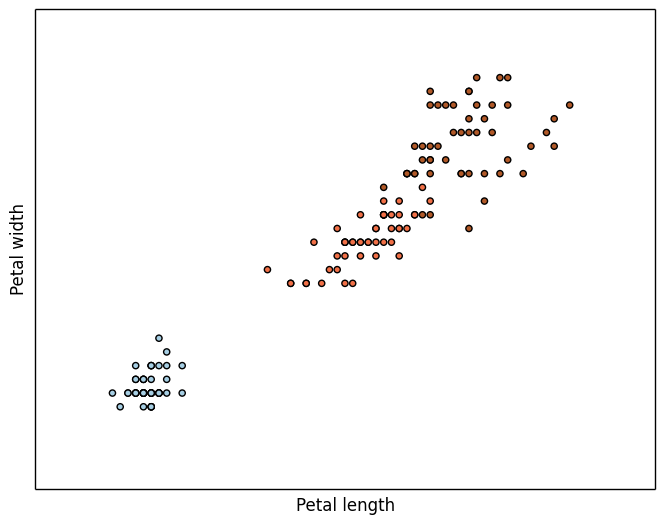
\includegraphics[scale=0.6]{images/petal_length-petal_width.png}
\end{figure}
\begin{figure}[!ht]
\centering
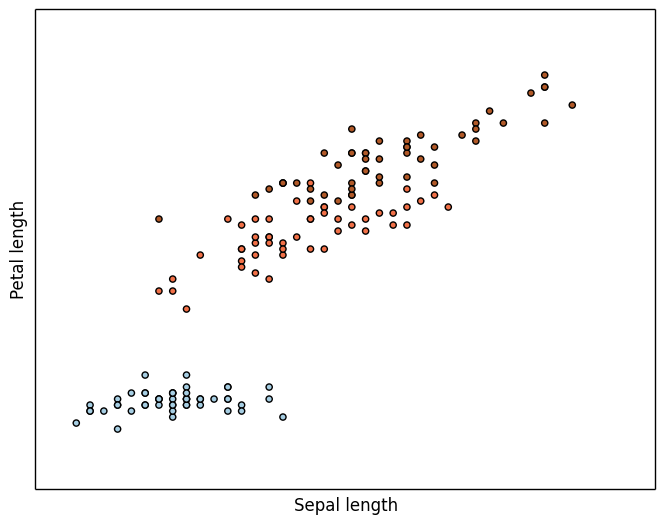
\includegraphics[scale=0.6]{images/sepal_length-petal_length.png}
\end{figure}
\begin{figure}[!ht]
\centering
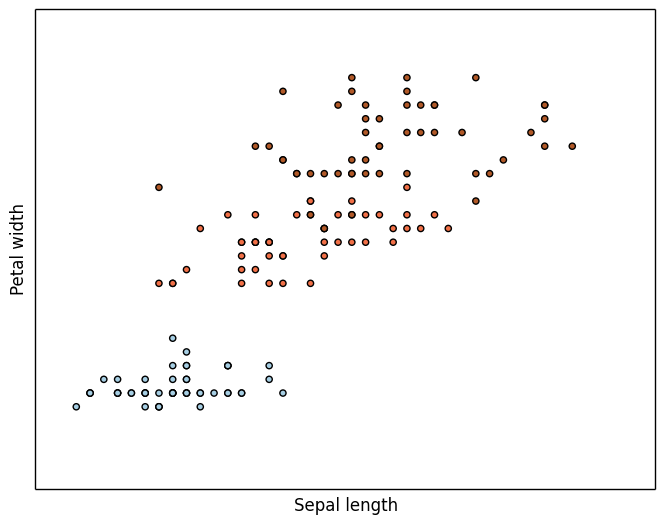
\includegraphics[scale=0.6]{images/sepal_length-petal_width.png}
\end{figure}
\begin{figure}[!ht]
\centering
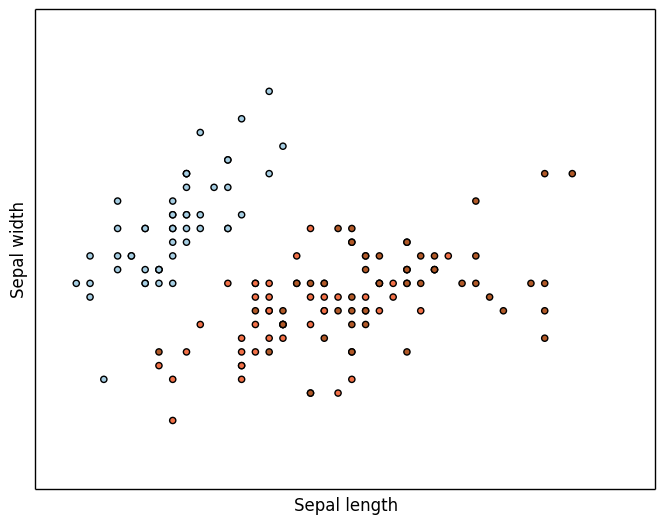
\includegraphics[scale=0.6]{images/sepal_length-sepal_width.png}
\end{figure}
\begin{figure}[!ht]
\centering
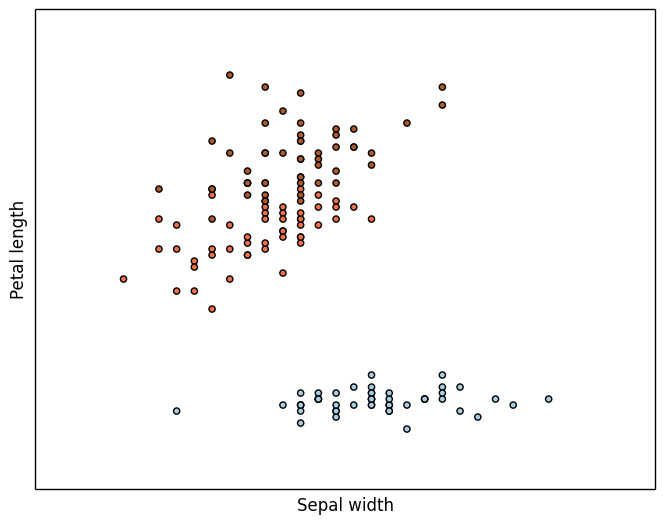
\includegraphics[scale=0.6]{images/sepal_width-petal_length.png}
\end{figure}
\begin{figure}[!ht]
\centering
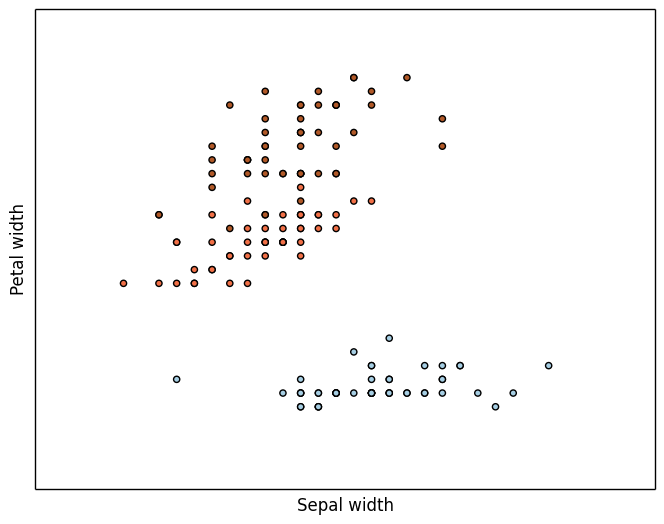
\includegraphics[scale=0.6]{images/sepal_width-petal_width.png}
\end{figure}

\clearpage
\bibliographystyle{plain}
\bibliography{bib}

\end{document}